\section{Analysis of first required behavior: Automatic vessel platform reconfiguration}
\label{analysisReconfiguration}

Automated modular vessel platform reconfiguration systems can be categorized as a more general "modular reconfigurable robot" system. 
Modular reconfigurable vessel systems can be evaluated from a non-maritime perspective, so where we are not directly focussing on vessels, but on more general modular reconfigurable robot (MRR) systems. \citet{seo2019modular} describes an MRR system as made up of many repeated modules (or units) that can be rearranged- or can rearrange themselves into different configurations depending on the task the robot is to solve at the time. The key characteristic of such systems is described as adaptability of hardware structure to suit a given task or environment. MRR systems differentiate themselves from normal robot systems by determining and executing a course of action, to change it's configuration. 

Various requirements of floating MRR systems were identified during the course of the project. Some approaches originating from sources about robotics in general were broader than approaches encountered in sources about modular vessel platforming. This section aims to conclude with two things. Firstly, it searches for fundamental characteristics of an automatic reconfiguring vessel platforming system. Secondly, the whole range of design choices and approaches is scoped down to a set that is expected to have the highest commercial feasibility. This is based on design choices of prior projects, supplemented with the authors argumented vision. 
During elaboration on system characteristics, prior projects will be discussed, more specifically, how they solved their challenges and in which characteristics did this result in. Automated vessel platform reconfiguration characteristics are discussed in 2 aspects; Strategies and Actuation. 



\subsection{Strategies}
\citet{yim2007modular} describes a taxonomy of architectures of modular robots, which is adopted to the use case of surface vessel platform reconfiguration. MRR system architectures are classified in three generally observed classes. They are described as follows \cite{yim2007modular}
\begin{itemize}
	\item \textbf{Lattice Reconfiguration Architectures} have units that are arranged and connected in some regular, three-dimensional pattern, resulting in a relatively simple and easily scalabe system. 
	\item \textbf{Chain or Tree Architectures} have	units that are connected together in a string or tree topology. This chain or tree can fold up to become space filling, but the underlying architecture is serial.
	\item \textbf{Mobile Architectures} have units that use the environment to maneuver around and can either hook up to form complex chains or lattices or form a number of smaller robots that execute coordinated movements and together form a larger	“virtual” network. 
\end{itemize}

We can see that \citet{o2014self} uses a lattice reconfiguration architecture in the horizontal surface plane (figure \ref{fig:wuh_assembly_planning}). Roboat shows L configurations in various publications, which can be considered a chain architecture, as configurations are used that do not fit in a repeating (lattice) pattern. Roboat reduces the amount of possible configurations by utilizing the square shape of the vessels to reduce the amount of orientations to steps in relative angle of 90 degrees.

Another classification can be found in the way structures are (re)configured. \citet{yim2007modular} distincts two approaches:
\begin{itemize}
	\item \textbf{Deterministic Reconfiguration} uses modules that are purposely manipulated to a target location.
	\item \textbf{Stochastic Reconfiguration} relies on statistics of a set of modules to configure in a more desirable configuration. System design is aimed to reach acceptable configuration without the need of predefined reconfiguration planning.
\end{itemize}

Stochastic reconfiguration can be achieved with very limited functionality per module. Due to robot simplicity, this approach can very desirable on micro scale which can be scaled to great numbers.
Deterministic reconfiguration needs more functionality embedded in a module. This system requires an agent that makes some form of plan, which is then to be executed. As a plan is formed and executed, this approach does give the opportunity to give more guarantees that a desired configuration is reached within a timespan. 

Due to technological advances, communication and computational hardware has become increasingly affordable. If the amount of modules in a system is relatively small, then equipping each individual with communication, computation and control systems is feasible. This allows creation of networks of robots that can share information, collaborate, negotiate and utilize benefits of all sorts of layered control architectures. Both \citet{o2014self} and Roboat utilize a deterministic approach to reach assembly. 

A common approach to solving the task of deterministic reconfiguration is dividing it in several tasks. \citet{o2014self} describes the following states to reach assembly:

\begin{itemize}
	\item Generation of desired configuration. \citet{o2014self} describes the result as a blueprint with a map of relative boat positions. 
	\item Connecting sequence selection. An entity selects a sequence in which the assembly is to happen. 
	\item Positioning of a module.  A trajectory of a vessel to an assembly location is generated and realized by actuators. 
	\item Docking Sequence. As a vessel reaches a docking site within an area of acceptance, the docking sequence runs, which should finalize the docking of that vessel. 
\end{itemize}

\citet{o2014self} greatly illustrates how they formulated strategies for generating connection sequence and module positioning (figure \ref{fig:wuh_assembly_planning} and \ref{fig:wuh_assem_approach})
 \begin{figure}[h!]
	\centering
	\makebox[\textwidth][c]{
		\begin{minipage}{0.45\textwidth}
			\centering
			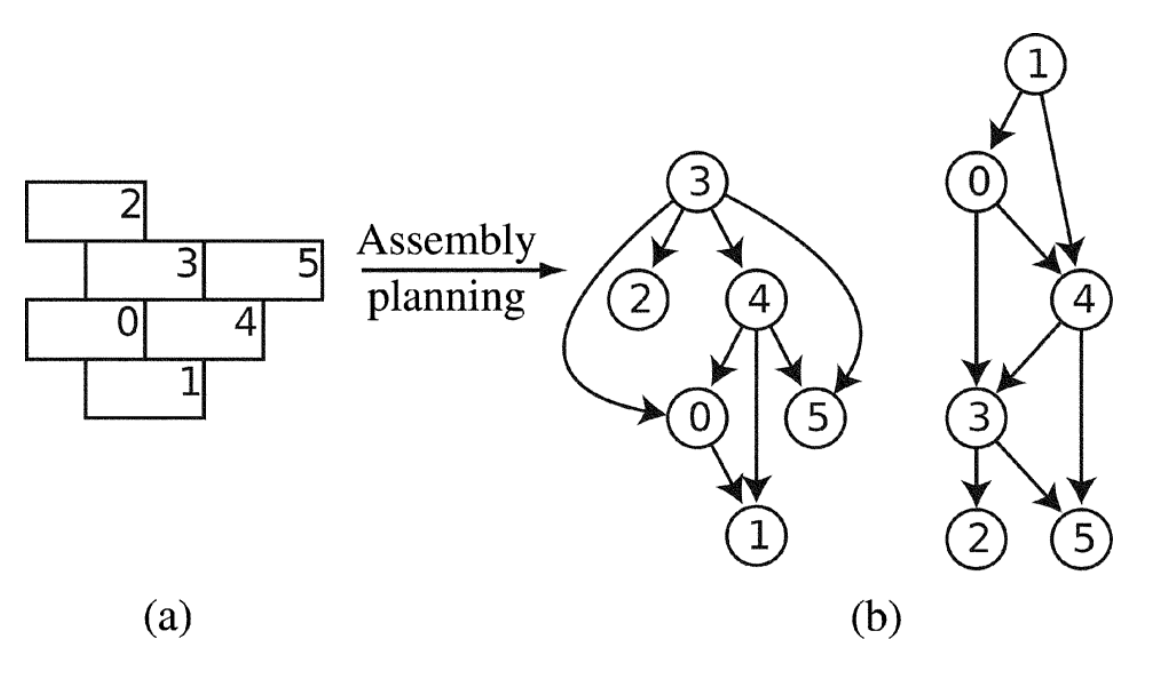
\includegraphics[width=0.95\textwidth]{img/wuh_assembly_planning}
			\caption{The assembly planning stage of \citet{o2014self}, showing desired platform blueprint (a) and two cannidate assembly sequences (b).}
			\label{fig:wuh_assembly_planning}
		\end{minipage}\hfill
		\begin{minipage}{0.45\textwidth}
			\centering
			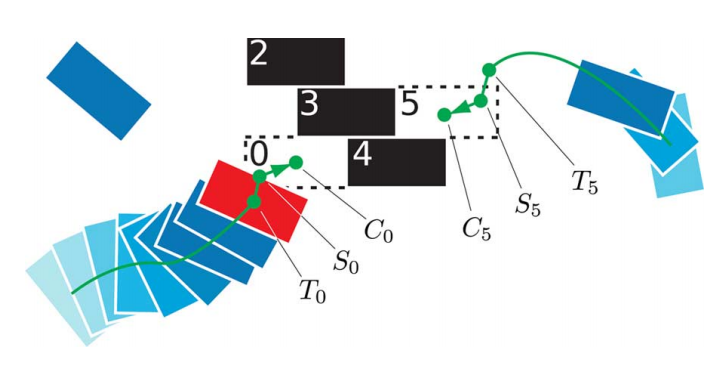
\includegraphics[width=0.95\textwidth]{img/wuh_assem_approach}
			\caption{The trajectory of assembling modules positioning to continue into a docking sequence \cite{o2014self}.}
			\label{fig:wuh_assem_approach}
		\end{minipage}
	}
\end{figure}

\subsection{Actuation}
Two tasks are identified that must be realized by actuators of the system:
\begin{itemize}
	\item means of relative repositioning modules during reconfiguration
	\item means of maintaining acceptable relative position between modules when connected
\end{itemize}

Altough these tasks can theoretically be done by a single system, \citet{seo2019modular} notices that MRR modules generally have two actuator systems to adress these tasks; a large main actuator to move itself with respect to other modules, and a smaller actuator that connects or disconnect two modules. 

The main actuator of MRR systems can be measured in nondimensional characteristic length, being "the number of modules that can be supported in a cantilever fashion under gravity"\cite{seo2019modular}. This measure is perhaps useful for some robotic systems, but does not make sense to use for vessel platforming systems, as gravitation is cancelled out by buoyancy and hydrodynamic forces. These forces are defined as \citet{fossen2011handbook}:
\begin{itemize}
	\item Buoyancy force due to the hydrostatic pressure (proportional to the displacement of the ship).
	\item Hydrodynamic force due to the hydrodynamic pressure (approximately proportional to the square of
	the relative speed to the water).
\end{itemize}

Vessel platforms are not considered excelling at tasks that require large speeds, but rather tasks that benefit from versatility, robustness  and low cost\cite{seo2019modular}. Vessels platforms with relatively low operational speeds can be classified as "Displacement Vessels" \citet{faltinsen2005hydrodynamics}
\begin{equation}
	Fn =  \frac{U}{\sqrt{gL}} < 0.4 \mbox{ }\mbox{ }\mbox{ }\mbox{ for vessels categorized as "Displacement Vessels"}
\end{equation} 

The nature of displacement vessels allow horizontal movement of masses (the ship itself and cargo) much higher with respect to robotic systems that lift, which results in a completely different order of magnitude of the ratio between propulsion and inertia. 
Vessel modules do need means of relocation with respect to other vessels with enough strength to overcome reasonable disturbances, such as wind or current. Further increasing the magnitude of forces that relocate the module reduces the achievable time that a module needs to relocate, which is also dependent on inertia and drag. Strength of main actuator and module mass are affected by various design choices, but optimal choices vary widely per use case. 
Systems that fulfull the task of moving the vessel in the surface plane come in many forms and configurations. Common actuators are propellers, rudders or fins. It is often considered desirable to have a set of actuators that allow imposing forces on all the three degrees of freedom independently, such that we can consider the module fully actuated. Figure \ref{fig:roboatAllocation} and \ref{fig:modularContainerAssembly} show actuator setups of the Roboat and \citet{o2014self}, which can both be considered fully actuated. 

 \begin{figure}[h!]
	\centering
	\makebox[\textwidth][c]{
		\begin{minipage}{0.45\textwidth}
			\centering
			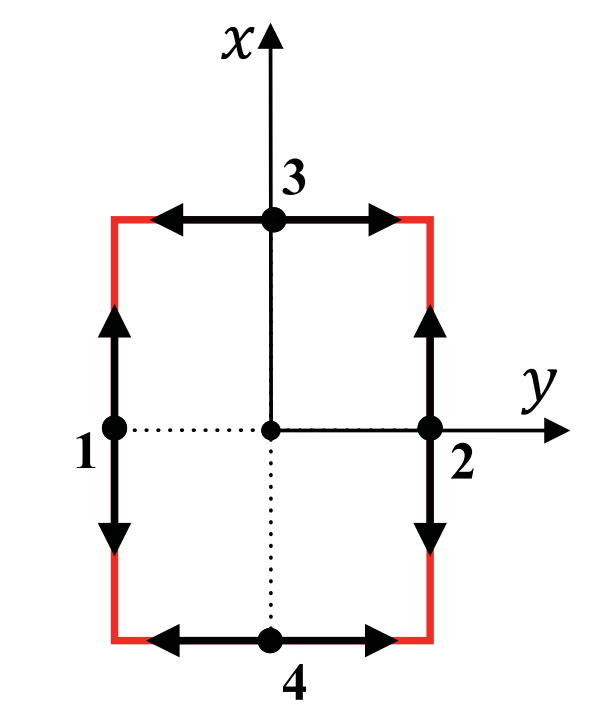
\includegraphics[width=0.75\textwidth]{img/roboatThrusterAllocationPlus}
			\caption{The "+" shaped thruster setup of Roboat \cite{wang2018design}}
			\label{fig:roboatAllocation}
		\end{minipage}\hfill
		\begin{minipage}{0.45\textwidth}
			\centering
			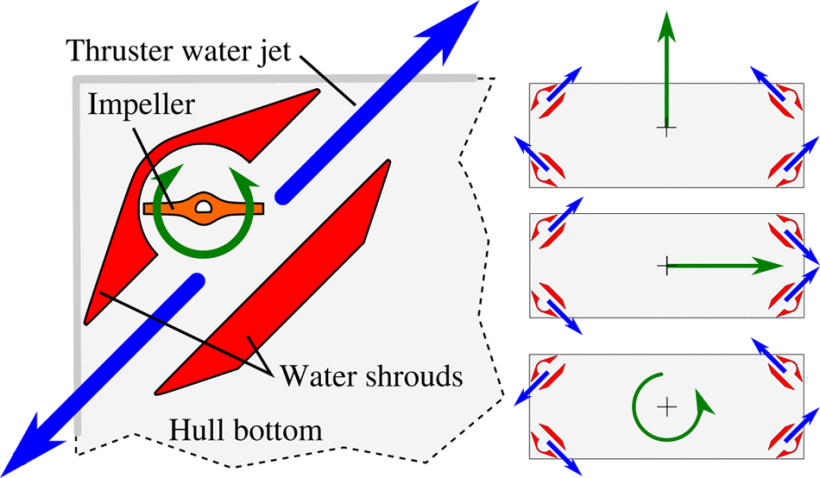
\includegraphics[width=0.9\textwidth]{img/TEMPMThrusterAllocation}
			\caption{The "x" shaped hruster setup of "Tactically expandable maritime platform module" \cite{o2014self}}
			\label{fig:modularContainerAssembly}
		\end{minipage}
	}
\end{figure}

A vessel platforming system needs means to maintain its configuration, which can be achieved using physical restraints that limit relative motion between modules for some period of operation. Movement of the platform as a whole can be desired, for instance when a vessel platform is performing a task of moving to a certain point or orientation. Undesired movement can be caused by disturbances. Alhough maintaining configuration of a vessel platform can theoretically be realized by the main actuators of the module, it is often seen that a second type of actuator is applied, specifically designed to reduce unwanted relative motion between modules by means of physical constraint. Generally once such systems are implemented, often by  mechanical \cite{mateos2019autonomous} \cite{o2014self} or magnetic \cite{kelly2019algorithms} means, the configuration is considered an assembly.


The application of MRR systems on vessel platforms is a niche which generally has specific goals, constraints, environments. The majority of the motion is on the surface plane, often allowing engineers to consider only three degrees of freedom. The environment already enforces some degree of dampening to the system, as various hydrodynamic dampening effects are always present on ships. Robots performing self-reconfiguration is a big topic, on which the most relevant concepts for vessel platforming are elaborated in this section. For further reading on general (not vessel platforming) MRR systems, consider \citet{yim2007modular} and \citet{seo2019modular} and references therein.



%"A key ability of MRR systems that differentiates them from normal robot systems is the
%This problem is referred to as
% and control." 


%More connecting methods can arise in the future, which do not fit a particular mentioned group. Hybrid systems are possible and can even %be more suitable to best exploit benefits of MRR systems for a particular application. 

%We consider a vessel system that self assembles a system with a connection mechanicm able to meet all prerequisites for this connecting mechanism to maintain acceptable relative motion. 
%Motion between connected vessels may be non neglectable, as was assumed in the case of \citet{paulos2015automated}. Their rope-like connections could change their stiffness by controlling tension in the cables that are part of their construction. The area of acceptance has been predicted and compared with success rate in their experimental setup. The connection protocol required the connecting vessels to be in constant relative position of one another. 


%\citet{mateos2019autonomous}'s ball joint connections between assembling vessels have a higher translational stiffness with respect to \cite{paulos2015automated}. The ball joints do however give almost no rotational stiffness between vessels. The ball joint latching system needs both vessels to approach one another at a small range of angles. the cone around the ball joint system helps to enlarge the area of acceptance, by physically guiding the relatively small joints to eachother. 


%Practically, both systems were able to perform vessel self assembly. Both systems will have benefits over one another, and there are even more solutions possible than the two described above. Choice of connection method and protocol is up to a designer, and optimal choices vary among applications. 

%What 



%\citet{seo2019modular} 


%\citet{seo2019modular} states: 
%"Here we will give examples of MRR systems in each architectural class. The intent is not to be exhaustive, but to find historically early %representative examples.
%"


%todo: map functions of the system. What is to be controlled and what not? There are more control tasks than generic ship control systems, which are to be discussed. 

%This section will discuss functions of general vessel systems. 
%Automation will be evaluated in four classes of functions as \citet{parasuraman2000model}. The classes of functions are as follows:
%\begin{enumerate}
%	\item information acquisition
%	\item information analysis
%	\item decision and action selection
%	\item action implementation
%\end{enumerate}
%Each of these functions can be automated independently. 

%In the context of 'ship control automation', the main function of a vessel system is considered the control of actuators to move the vessel. Operation of other functions are usually not the main focus. 
%A vessel controller able to realize a ship performing a succesful voyage might not be designed for loading and unloading a vessel, mainenance or fuel management.

%Vessel control systems can be equipped to manage tasks other than moving the vessel depending, but the core function usually contains motion control. 

%Generally communication, maintenance and other non manouvering jobs are not the scope when determining wether a vessel is automated or not. The nature of the controller of the ship's propulsion system determines automation. 

%Control may be achieved with a variety of systems that operate on different levels. 
%Consider a first system: Heading control of a vessel, achieved with a PID controller. Only one actuator (rudder) is controlled. The system controls actuation of the rudder, according to predefined laws for that operation. 
%Consider a second system: A vessel-system plans it's trajectory in a dynamic environment to arrive at a given destination, and controls actuators to realize this. 

%With respect to the former, system two will be more layered, equipped with more, sensors, actuators, and protocols, potentially performing more complex tasks. Yet, both systems have a controller that is responsible for a set of actuators. Both controllers decide and realize actuation for a given time. 
%-----

% DOUBLE ! \subsection{System A: automatic vessel platform assembly}
%With respect to the function of vessel motion control, another system function emerges in vessel platforming; assembly. 

%This means we are looking to automate vessels such that a present connecting system able to, partially or completely, prevent motion between vessels, thus forming a single body. Systems that connect vessels have requirements to perform reliably. The need of a specific relative motion between vessels varying over a connection-period is common, if not a must. 

%If the connection protocol was succesful, relative motion between vessels is restricted to some degree, or up to certain limits. Connections can be modeled as springs. Connectors with stiffness so high that relative motion between vessels 

% What does it mean to become a platform? What does this require?
%To consider vessels a platform, a method of connecting is required. This should be any tool that restricts or prevents relative motion between modules, up to certain limits. This can be of mechanical nature \citet{mateos2019autonomous}, or other means, such as with springs or magnets. % Roboat latching paper

%To call a system self-assembling: what is required?
%We need a vessel system that can manage orienting the vessel to come in range of acceptance of a connecting mechanism, as described above. Furthermore the ships need to satisfy demands that result from the specific latching system, such as time or contact force. 

%The self assembling features of a vessel system can generally be evaluated with indicators such as speed, reliability, energy consumption wear and ease of use, according to the demands of a use case. 
